\chapter{Einleitung}

\begin{fquote}[Mark Zuckerberg][Facebook CEO][2014]
Virtual reality was once the dream of science fiction. But the internet was also once a dream, and so were computers and smartphones. The future is coming.
\end{fquote}

\begin{fquote}[Tim Cook][Apple CEO][2017]
I think AR is [...] big, it’s huge. I get excited because of the things that could be done that could improve a lot of lives.
\end{fquote}

\section{Einführung}
Viele der einflussreichsten Technologieunternehmen arbeiten an der \emph{Virtual} bzw.\ \emph{Augmented Reality (VR} bzw.\ \emph{AR)}. Tim Cook ist überzeugt davon, dass die AR die nächste \emph{``big idea''} nach dem Smartphone wird \cite{theindependent2017apple}.

Nicht nur Großkonzerne wie Apple, Facebook oder Samsung arbeiten intensiv in diesem Bereich. Ein Start-up-Unternehmen namens \emph{Magic Leap} entwickelt eine AR Brille und wird von Investoren in Billionenhöhe unterstützt \cite{kelly2016untold}. Laut einem Cover-Artikel der Zeitschrift \emph{Wire} ist die noch unter Verschluss gehaltene Technologie den Konkurrenzprodukten allen voraus. Das Release der Hardware ist Stand heute noch nicht bekannt, aber es lässt sich ein Trend erkennen, der die nächsten Jahre viele neue Möglichkeiten eröffnen wird und möglicherweise die Digitalisierung revolutionieren könnte.
Diese Arbeit wird sich mit einer Anwendung für die AR beschäftigen -- der Softwarevisualisierung. Die Spezialisierung auf AR kann nach der Abgrenzung von AR und VR besser nachvollzogen werden.

\paragraph{VR} ist eine Umgebung, in der der Betrachter vollkommen von einer computergenerierten Welt umgeben ist, die oft die reale Welt imitiert, aber auch rein fiktiv sein kann \cite{milgram1995augmented}.\\

Obwohl der Begriff AR zunehmend in der Industrie Verwendung findet, entbehrt er doch einer einheitlichen Definition. In \cite{azuma1997survey} wird AR als \emph{"`Variation"'} von VR betrachtet. Dagegen vermittelt Milgrim in \cite{milgram1995augmented} ein vollständigeres Verständnis, weshalb sich die Begrifflichkeiten in dieser Arbeit daran anlehnen sollen. Nach Milgrim existieren die beiden entgegengesetzten Extreme der Realität und der Virtualität. Alles dazwischen ist die sogenannte \emph{Mixed Reality (MR)}.

\paragraph{MR} ist eine Umgebung, in der Elemente der realen und einer virtuellen Welt zusammen dargestellt werden \cite{kato1999marker}.\\

\begin{figure}[htb]
  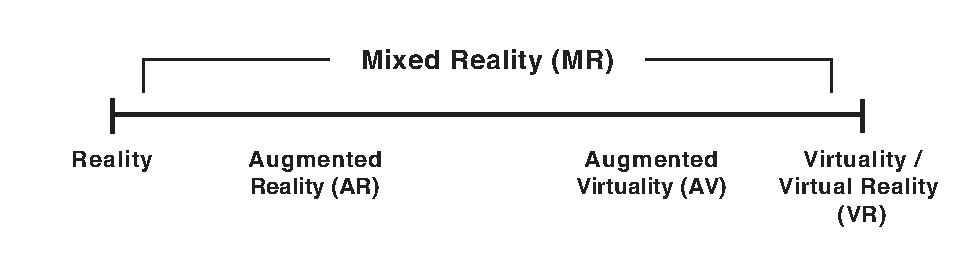
\includegraphics[width=.8\textwidth]{\figdir/rv-continuum}
  \caption{Abgewandelte Darstellung des Reality-Virtuality-Kontinuums aus \cite{milgram1995augmented}}
  \label{fig:rv-continuum}
\end{figure}

Dieses \emph{Reality-Virtuality-Kontinuum} ist in Abbildung \ref{fig:rv-continuum} dargestellt, in dem gut zu erkennen ist, dass AR zu der Mixed Reality gehört. In den meisten Quellen wie \cite{azuma1997survey, azuma2001recent, kato1999marker} wird bei der AR noch die Komponente der Interaktion aufgeführt. AR kann deshalb folgendermaßen definiert werden:

\begin{defbox}{AR}{ar}
   AR ist die Erweiterung der realen Welt durch computergenerierte Elemente, mit denen der Betrachter in Echtzeit interagieren kann.
\end{defbox}

Auch die \emph{Augmented Virtuality}, also die Erweiterung der virtuellen Welt durch reale Elemente, gehört zur MR.

Wie viele der einflussreichsten Menschen der Technologie-Industrie, sieht Tim Cook  mehr Zukunft in der AR, da, wie er in einem Interview sagt, diese Technologie nicht wie die VR die wirkliche Welt ausschließt, sondern die Realität erweitert und Teil von zwischenmenschlicher Kommunikation sein kann \cite{theindependent2017apple}.

Wir stellen uns ein Hologramm vor, dass auf einem Konferenztisch Gestalt annimmt und ein Software-System repräsentiert. Entwickler, Projektleiter oder auch Kunden versammeln sich um den Tisch und können miteinander interaktiv die Software betrachten, evaluieren und wichtige Informationen daraus ziehen.

Dies wäre mit VR nicht möglich, da der Betrachter von der Außenwelt abgeschottet ist. Deshalb wird im Zuge dieser Arbeit mit der Stand heut am weitesten ausgereiften Technologie der AR gearbeitet -- der \emph{HoloLens} von Microsoft.

\section{Motivation dieser Arbeit}
Die Technologie der AR bietet uns viele neue Möglichkeiten. Eine Motivation dieser Arbeit ist es sich produktiv mit einer neuen, zukunftsträchtigen Technologie zu beschäftigen. Das ist jedoch nur die eine Seite. Die weitaus größere Motivation ist, die zuvor noch nicht dagewesene Zugänglichkeit und Interaktion mit dreidimensionaler \emph{Visualisierung} auszunutzen. Visualisierung im Allgemeinen begegnet uns in vielen Bereichen unseres Lebens und nimmt eine wichtige Rolle ein.

Niemand konnte bislang unser Sonnensystem von außen betrachten. Dennoch haben wir alle eine ziemlich gute Vorstellung wie dieses aufgebaut ist. Durch die Visualisierung der Planeten und der Sonne entsteht in uns ein geistiges Abbild der Realität. Das Konzept komplexe Realitäten zu abstrahieren und zu visualisieren, um dadurch die Realität besser verstehen zu können, ist in vielen Disziplinen der Wissenschaft vertreten.

Neben Wissenschaften wie Physik, Chemie oder Biologie, nimmt Visualisierung
auch besonders in der Informatik eine wichtige Rolle ein. In vielen Bereichen müssen Informationen in eine visuelle Form gebracht werden, die für das menschliche Auge besser zu lesen sind.

Gerade bei komplexen Software-Systemen ist das der Fall. Soll zum Beispiel die zu Grunde liegende Struktur einer Software Außenstehenden erklärt werden, gelingt das mit einem visuellen Modell wie einem UML-Diagramm sicherlich besser, als nur in den Source-Code zu schauen.

So wie UML-Diagramme, war die Darstellungsform der Softwarevisualisierung bislang meist zweidimensional. Mit AR wird dieser Disziplin der Visualisierung jedoch wortwörtlich ein neuer Raum an Möglichkeiten eröffnet und in diese Arbeit soll diesen Raum ausfüllen.

\section{Zielsetzung}
Für die Zielsetzung einer 3D Softwarevisualisierung in der AR sollten zunächst die allgemeinen Ziele einer Softwarevisualisierung betrachtet werden. Softwarevisualisierung ist für Diehl die "`visualization of artifacts related to software and its development process"' \cite{diehl2007software}. Wird der Fokus mehr auf die Ziele, d.h. den Nutzen für den Betrachter gelegt, lässt sich Softwarevisualisierung wie folgt definieren:

\begin{defbox}{Softwarevisualisierung}{software-visualization}
Softwarevisualisierung ist die bildliche oder auch metaphorische Darstellung einer Software, um dem Betrachter durch Vereinfachung und Abstraktion das bessere Verständnis oder die einfachere Analyse von Software zu ermöglichen.
\end{defbox}

In dieser Arbeit soll das neue Konzept \emph{CodeLeaves} für eine solche Softwarevisualisierung in der AR vorgestellt und im Detail ausgearbeitet werden.

Dabei soll CodeLeaves, im Vergleich zu andern 3D Softwarevisualisierungen, die Vorteile der Dreidimensionalität optimal ausnutzen.

Im Vorfeld dieser Arbeit wurden in einer Studie Metriken gesammelt, die eine gute Softwarevisualisierung bzw. CodeLeaves unterstützen sollte.

Es sollen dynamische und statische Metriken zur Erkennung von Anomalien in einer Software unterstützt werden. Ebenfalls soll die Darstellung der Struktur und der darauf abgebildeten Abhängigkeiten innerhalb einer Software möglich sein.

Durch weitere Expertengespräche sollen Userstories erstellt werden um den Mehrwert des neuen Konzepts validieren zu können.

Um diesen Anforderungen gerecht zu werden, soll für CodeLeaves ein sprachunabhängiges Datenmodell entworfen werden, dass alle geforderten Metriken unterstützt.

Der Praktische Teil dieser Arbeit soll die prototypische Entwicklung von CodeLeaves für die HoloLens sein.

\section{Aufbau der Arbeit}
Im Kapitel \ref{ch:concept} wird das Konzept von CodeLeaves vorgestellt. Dabei wird zunächst unter Betrachtung alternativer Ansätzen begründet, wieso ein neues Konzept sinnvoll ist, um dann in Abschnitt \ref{sec:idea} genauer auf das Konzept einzugehen. Die Befragung von Experten der Softwareanalyse und die daraus abgeleiteten Anforderungen an CodeLeaves in Abschnitt \ref{sec:requirements} schließen das erste Kapitel ab.

Das Kapitel \ref{ch:data-model} beschäftigt sich mit der Entwicklung eines geeigneten Datenmodells für CodeLeaves. Es werden vorhandene Datenmodelle auf Tauglichkeit für CodeLeaves überprüft und Rücksprache mit erfahrenen Software-Ingenieuren gehalten.

Aufbauend auf das entwickelte Datenmodell, wird das Konzept von CodeLeaves in Kapitel \ref{ch:modelling} theoretisch weiter ausgearbeitet. Darunter fällt die Positionierung der Bäume auf einer Grundfläche und die Länge, Dicke und der Winkel der einzelnen Äste. Parallel zur Theorie wird aufgezeigt, wie sich CodeLeaves in Unity für die HoloLens modellieren lässt.

Die Interaktion mit CodeLeaves soll Thema des Kapitel \ref{ch:interaction} sein. Besonders die Abhängigkeiten von Artefakten einer Software sollen mithilfe von CodeLeaves interaktiv exploriert werden können.

Das Kapitel \ref{ch:conclusion} fasst die Ergebnisse der Arbeit zusammen und ein Ausblick auf zukünftige Verwendung und weiterführende Arbeiten runden die Arbeit ab.

\chapter{Das Konzept CodeLeaves}
\label{ch:concept}

\section{CodeLeaves und die Metapher Software-Wald}
\label{sec:idea}

\emph{``Hierarchies are almost ubiquitous [...]''} \cite{robertson1991cone} halten Robertson \emph{et al.}
 schon 1991 bei der Visualisierung von hierarchischen Informationen fest. So auch bei der Struktur einer Software. Jede Software mit einer geschachtelten Paketstruktur ist hierarchisch und kann in einer Baumstruktur dargestellt werden. \emph{"`Bäume sind eine der wichtigsten Datenstrukturen, die besonders im Zusammenhang mit hierarchischen Abhängigkeiten und Beziehungen zwischen Daten von Vorteil sind."'} \cite{ernst2016grundkurs} stellen auch Ernst \emph{et al.} fest. Draus folgt, dass die Darstellung von Software als Baum oder auch Bäume sinnvoll ist.

Der Baum in der Informatik zeugt von einer ursprünglichen Metapher -- der Baum, wie er draußen in der Natur wächst. Da dieser unbestritten dreidimensional ist, liegt eine Softwarevisualisierung für die Dreidimensionalität mit einer realitätsnäheren Interpretation der Baum-Metapher nahe. Werden die Bäume, die im zweidimensionalen meist von oben nach unten gezeichnet wird, in 3D in natürlicher Wuchsrichtung modelliert und mehrere Bäume für eine Software verwendet, entsteht eine neue Metapher: der \emph{Software-Wald}.

CodeLeaves stellt ein Konzept dar, dass sich die Metapher des Software-Waldes zu nutze macht und wird im Folgenden auf High-Level-Ebene skizziert und danach genauer erläutert:

\begin{titlebox}{\textbf{Konzept:} CodeLeaves}
  \begin{enumerate}
    \item Die Struktur der Software wird mit nach oben wachsenden Bäumen dargestellt.
    \item Jedes Paket im \emph{Root-Verzeichnis} wird als einzelner Baum auf einer Ebene -- dem \emph{Waldboden} -- dargestellt.
    \item Die Blätter der Bäume entsprechen den Softwareartefakten (z.B. Klassen) und können durch ihre Farbe eine beliebigen Metrik visualisieren. 
    \item Zwischen den Bäumen entsteht ein \emph{Wurzelgeflecht}, was die aggregierten Abhängigkeiten zwischen den Paketen darstellt.
    \item Abhängigkeiten oder Aufrufe zwischen einzelnen Softwareartefakten werden aggregiert über die Elternpakete als farbige bzw. Dicke der Äste dargestellt oder alternativ als direkte \emph{Spinnweben} zwischen den Bäumen.
  \end{enumerate}
\end{titlebox}

\paragraph{Punkt 1} ist dafür verantwortlich, dass die Softwarevisualisierung nahe an der tatsächlichen Software ist, wie sie ein Entwickler in seiner Code-Base gewöhnt ist. Das heißt, diejenigen, die auch tatsächlich mit der Software arbeiten, finden sich aufgrund der bekannten Baumstruktur auch in der Visualisierung schnell zurecht, ohne jedes Softwareartefakt auszuwählen, um zu sehen, mit welchem sie es zu tun haben. Im Fachjargon wird hier von der \emph{Habitability} gesprochen, also wie schnell oder gut sich ein Betrachter in einer Software oder auch deren Visualisierung "`zuhause"' fühlt \cite{wettel2007program}.

\paragraph{Punkt 2} ist weitgehend selbsterklärend. Durch Darstellung der Software in mehreren Bäumen entsteht erst der Software-Wald und die Pakete im Root-Verzeichnis als Wurzeln der Bäume zu verwenden bietet sich an. Das schließt jedoch nicht aus, dass Unterpakete als neuer Waldboden verwendet wird. Interaktion mit dem Waldboden soll Teil des Kapitel \ref{ch:interaction} sein.

\paragraph{Punkt 3} bedeutet, dass in CodeLeaves durch die Farbe der Blätter ein \emph{Laubdach} entsteht, dass eine gute Übersicht über eine ausgewählte Metrik der Software gibt. Beispielsweise kann der Farbe der Blätter die Code-Coverage der einzelnen Softwareartefakte (siehe Definition \ref{def:softartefact}) zugewiesen werden. Mit einer Skala von Grün bis Rot kann dann der Software-Wald bei guter Testabdeckung im sommerlichen Grün erstrahlen, oder bei einer weniger guten Coverage eher in den Herbst übergehen. Die Färbung des Laubdachs ist flexibel auf jegliche Metrik anwendbar, die bei der betrachteten Software zur Verfügung steht.

\begin{defbox}{Softwareartefakt}{softartefact}
  Ein Softwareartefakt wird in dieser Arbeit als Überbegriff für die kleinste betrachtete Einheit der Software verstanden. Das können bei objektorientieren Sprachen typischerweise Klassen, aber auch bei feinerer Granularität einzelne Funktionen innerhalb einer Klasse sein. Auch die Betrachtung von Dateien, die mehrere Klassen enthalten können, sind denkbar.
\end{defbox}

\paragraph{Punkt 4} bietet einen goßen Vorteil gegenüber der Zweidimensionalität. In Abbildung \ref{fig:3d-advantage} wird rechts das Prinzip des Wurzelgeflechts mit einem minimalistischen Beispiel illustriert.

\begin{figure}[htb]
  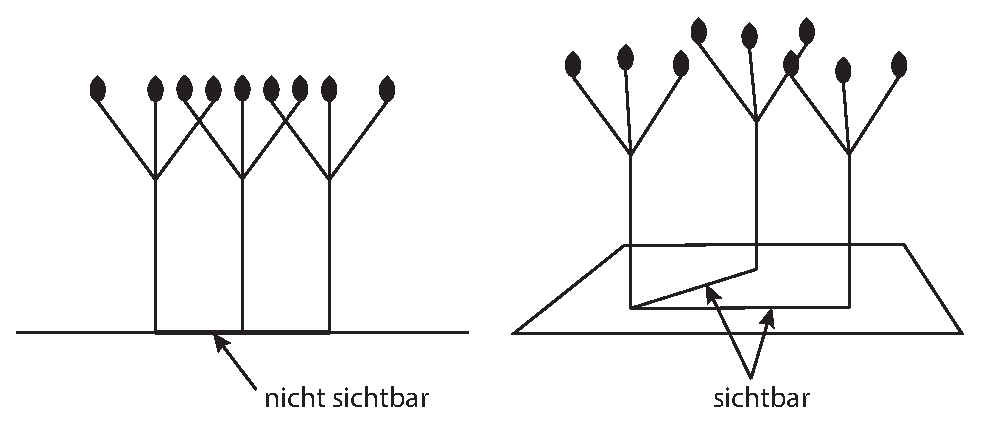
\includegraphics[width=.8\textwidth]{figures/3d-advantage}
  \caption{Vorteil der Dreidimensionalität bei der Darstellung von Abhängigkeiten}
  \label{fig:3d-advantage}
\end{figure}

Die Abhängigkeiten zwischen den Bäumen wird auf einen Blick ersichtlich. Betrachtet man die Bäume in 2D, wie es im linken Teil der Abbildung dargestellt ist, verschwinden die Abhängigkeiten hintereinander und sind nicht zuzuordnen.

\paragraph{Punkt 5} heißt, dass die Abhängigkeiten einer Software sehr übersichtlich auf die Struktur der Software abgebildet werden können, ohne diese zu beeinflussen. Für das besser Verständnis bedarf es einer Definition der Aggregation von Abhängigkeiteän.

\begin{splitbox}{Aggregation von Abhängigkeiten}{aggregation}
Bei der Aggregation von Abhängigkeiten zwischen Softwareartefakten werden die Abhängigkeiten nicht direkt dargestellt, sondern über die Eltern-Pakete geleitet. Seien $x, y$ Pakete und Softwareartefakt $A \in x$ besitze eine Abhängigkeit zu Softwareartefakt $B \in y$, dann geht die Abhängigkeit von $A$ zu einem zusätzlich Konstrukt $\Psi_x$, das das Pakets $x$ repräsentiert. Angenommen $x$ und $y$ befinden sich zudem im Paket $z$, dann geht die aggregierte Abhängigkeit entweder direkt von $\Psi_x$ zu $\Psi_y$, oder weiter über $\Psi_z$ zu $\Psi_y$ und schließlich $B$.
\tcblower
%\raggedright
%Beispiel in CodeLeaves:\par\vspace{.6cm}
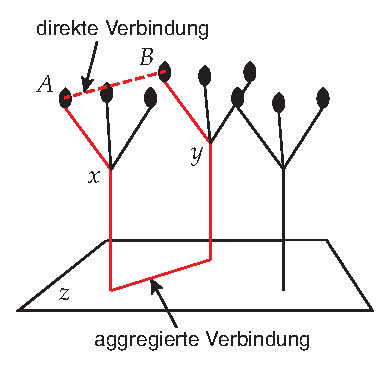
\includegraphics[width=\linewidth]{figures/aggregation}
\end{splitbox}

Auf der rechten Seite der Definition \ref{def:aggregation} ist eine aggregierte Abhängigkeit am Beispiel von CodeLeaves zu sehen. Die $\Psi$ in CodeLeaves sind die Knoten der Bäume, an denen die Äste zusammen laufen und im Spezialfall des Root-Verzeichnisses, der Waldboden.

Bei mehreren Abhängigkeiten zwischen Nachbar-Paketen, überlagern sich die aggregierten Abhängigkeiten zwangsläufig. Falls in unserem Beispiel eine weitere Abhängigkeit von Paket $x$ zu Paket $y$ bestünde, würden sich die Abhängigkeiten von $\Psi_x$ bis $\Psi_y$ überlagern. Daraus ergibt sich, dass nicht jede aggregierte Abhängigkeit ohne Interaktion zwangsläufig eindeutig zuzuordnen ist.

Wird aber bei jeder Kante, sei es ein Ast, Stamm, oder Wurzel, die Anzahl an überlagernden Abhängigkeiten als Dicke der Kante dargestellt, bekommt der Betrachter eine gute Übersicht über die Gesamtheit der Abhängigkeiten. Durch Interaktion mit einzelnen Kanten, oder sogar des ganzen Waldbodens, soll eine fein granulärere Analyse der Abhängigkeiten möglich sein.

Das zweite Element von Punkt 5 sind die Spinnweben. Damit lassen sich die Abhängigkeiten direkt darstellen. Um bei großen Software-Systemen aber die Übersicht über den Wald nicht zu verlieren, sollten diese mithilfe der Interaktion des Nutzers flexibel aktivierbar sein.

\section{Vergleich mit anderen Konzepten}
\label{sec:comparison}

Im Vorfeld dieser Arbeit wurde in \cite{puetz2017softwarevisualisierung} evaluiert, was eine gute Softwarevisualisierung ausmacht und unterstützen sollte. Ausgehend davon, wurden vorhandene 3D Visualisierungen und andere mögliche Konzepte miteinander verglichen. Die Ergebnisse dieser Untersuchung, soll in Folgenden vorgestellt werden.

Um herauszufinden welchen Mehrwert sich Nutzer einer Softwarevisualisierung von dieser versprechen, wurde eine Umfrage in der QAware GbmH durchgeführt. Die QAware ist ein Projekthaus mit den Kerngeschäften Diagnose, Sanierung, Exploration und Realisierung von Software \cite{qaware2017it-probleme}. Durch die Erfahrung in Projekten für namhafte Kunden, zeichnen sich die Mitarbeiter durch fundiertes Wissen und Expertise aus. Es wurden insgesamt 22 Mitarbeiter mit unterschiedlichen Rollen in der Softwareentwicklung befragt.

\begin{figure}[hbt]
\begin{tikzpicture}
  \begin{axis} [
    width = \textwidth,
    height = 8cm,
    symbolic x coords={Lines of Code, Komplexität, Coverage, Struktur, Abhängigkeiten, Code-Violations, Anzahl Aufrufe, Ausführungszeiten, Laufzeitfehler, Ressourcen-Auslastung, Evolution der Statik, Evolution eins Themas},
    xtick={Lines of Code, Komplexität, Coverage, Struktur, Abhängigkeiten, Code-Violations, Anzahl Aufrufe, Ausführungszeiten, Laufzeitfehler, Ressourcen-Auslastung, Evolution der Statik, Evolution eins Themas},
    x tick label style={rotate=45, anchor=east, align=center},
    major x tick style = transparent,
    axis lines = left,
    axis line style = {-},
    ymajorgrids = true,
    ylabel=Anzahl,
    legend style = {at={(.99,.98)}, anchor=north east, legend columns=-1, column sep=1ex},
    ymin=0,
    bar width=5mm,
    ybar=-0.5cm,
    enlarge x limits={abs=0.6cm}
  ]
    \addplot[style={fill=primary}]
      coordinates {(Lines of Code, 1) (Komplexität, 3) (Coverage, 1) (Struktur, 5) (Abhängigkeiten, 7) (Code-Violations, 4)};
    \addplot[style={fill=secondary}]
      coordinates {(Anzahl Aufrufe, 5) (Ausführungszeiten, 5) (Laufzeitfehler, 1) (Ressourcen-Auslastung, 1)};
    \addplot[style={fill=tertiary}]
      coordinates {(Evolution der Statik, 3) (Evolution eins Themas, 1)};

    \legend{Statik, Dynamik, Evolution}

  \end{axis}
\end{tikzpicture}
\caption{Von Mitarbeitern der QAware gewünschte Informationen} \label{fig:survey}
\end{figure}

In Abbildung \ref{fig:survey} ist zu sehen, wie oft welche Metriken genannt wurden. Alle Metriken lassen sich in die drei Kategorien der Softwarevisualisierung aus \cite{diehl2007software} einordnen und sind farbig entsprechend gruppiert.

\paragraph{Statik} sind die Informationen, die ohne die Ausführung der Software generiert werden können \cite{diehl2007software}. Darunter fallen die Metriken, die als Zahl zu jedem Softwareartefakt zugeordnet werden können und damit zueinander in Relation gesetzt werden können. Genannt wurden LOC, Komplexität, Coverage und Code-Violations. Letzteres sind beispielsweise Verletzungen von vereinbarten \emph{Code-Conventions}. Die Informationen, die komplizierter zu visualisieren sind, stellen die Struktur und die Abhängigkeiten dar. Aus Abbildung \ref{fig:survey} geht hervor, dass diese Informationen gleichzeitig am meisten von Interesse sind.

\paragraph{Dynamik} beschreibt die Informationen, die zur Laufzeit einer Software generiert werden können \cite{diehl2007software}. Besonders oft wurden Ausführungszeiten von Softwareartefakten und Anzahl von Aufrufen genannt. Damit sind beispielsweise \emph{Bottlenecks} identifizierbar. Auch die Darstellung der Laufzeitfehler einer fehlerhaften Software sind für deren Analyse wichtig. Die Resourcen-Auslastung ist dabei auch hilfreich, wirkt sich jedoch wenig auf das 3D Modell der Softwarevisualisierung aus, da diese Informationen parallel zur eigentlichen Software existieren.

\paragraph{Evolution} beschreibt den zeitlichen Verlauf einer Software und stellt den Entwicklungsprozess in den Vordergrund \cite{diehl2007software}. Beispielsweise kann die Entwicklung statischer Metriken verfolgt werden. Mit der Evolution eines Themas ist gemeint, dass anhand die Entwicklung eines bestimmten Themas nachverfolgt werden kann.\\

Aus den von den Mitarbeiten gewünschten Informationen und weitern Rahmenbedingungen wurde in \cite{puetz2017softwarevisualisierung} folgende Kriterien aufgestellt, anhand derer vier verschiedene Modelle der 3D Softwarevisualisierung bewertet wurden.

\begin{itemize}
  \itemsep0pt
  \item Statische Metriken (z.B. Komplexität)
  \item Struktur
  \item Abhängigkeiten
  \item Dynamik (Primär Ausführungszeiten und Anzahl der Aufrufe)
  \item Evolution
  \item Habitability (vgl. Kapitel \ref{ch:concept} Punkt 1)
  \item Drilldown
  \item Technische Machbarkeit
\end{itemize}

Bei dem Kriterium Drilldown wurde bewertet, wie gut eine Visualisierung ihre Informationen von High-Level, bis hin zu Details darstellen kann.

Bei der technischen Machbarkeit wurde berücksichtigt, ob eine existierende Softwarevisualisierung für die HoloLens verwendbar ist. In Abbildung \ref{fig:alternatives} sind die untersuchten Alternativen abgebildet, darunter auch ein erster Entwurf von CodeLeaves.

\subsubsection*{CodeCity}
2007 stellten Wettel et al. CodeCity vor, die mithilfe der \textit{Stadt-Metapher} dreidimensionale Städte visualisiert, in denen Klassen als Gebäude und Pakete als Stadtviertel dargestellt werden \cite{wettel2007program, wettel2008visual, wettel2011software}. Für die Breite und Tiefe der Gebäude wurde für die Anzahl der Attribute (engl. \emph{number of attributes (NOA)}) und für die Höhe die Anzahl der Methoden (engl. \emph{number of methods (NOM)}) der visualisierten Klasse gewählt.

Die CodeCity ist als Konzept sehr durchdacht, bietet durch die Metapher gute Habitability und unterstützt die Darstellung der Evolution. Auch soll nach Wettel et al. die CodeCity die Analyse von Software im Vergleich zu herkömmlichen Analyse-Werkzeugen signifikant verbessern \cite{wettel2011software}.

Jedoch unterstützt CodeCity keine Dynamik und die Abhängigkeiten sind nur als direkte Verbindungen darstellbar, was bei größeren Software-Systemen sehr unübersichtlich wird. Die verfügbaren statischen Metriken sind begrenzt und vor allem ist die Technologie Stand heute nicht mehr produktiv einsetzbar \cite{puetz2017softwarevisualisierung}.

\newlength\fwidth
\setlength{\fwidth}{.49\textwidth}
\begin{figure}[htb]
  \centering
  \begin{subfigure}[b]{\fwidth}
   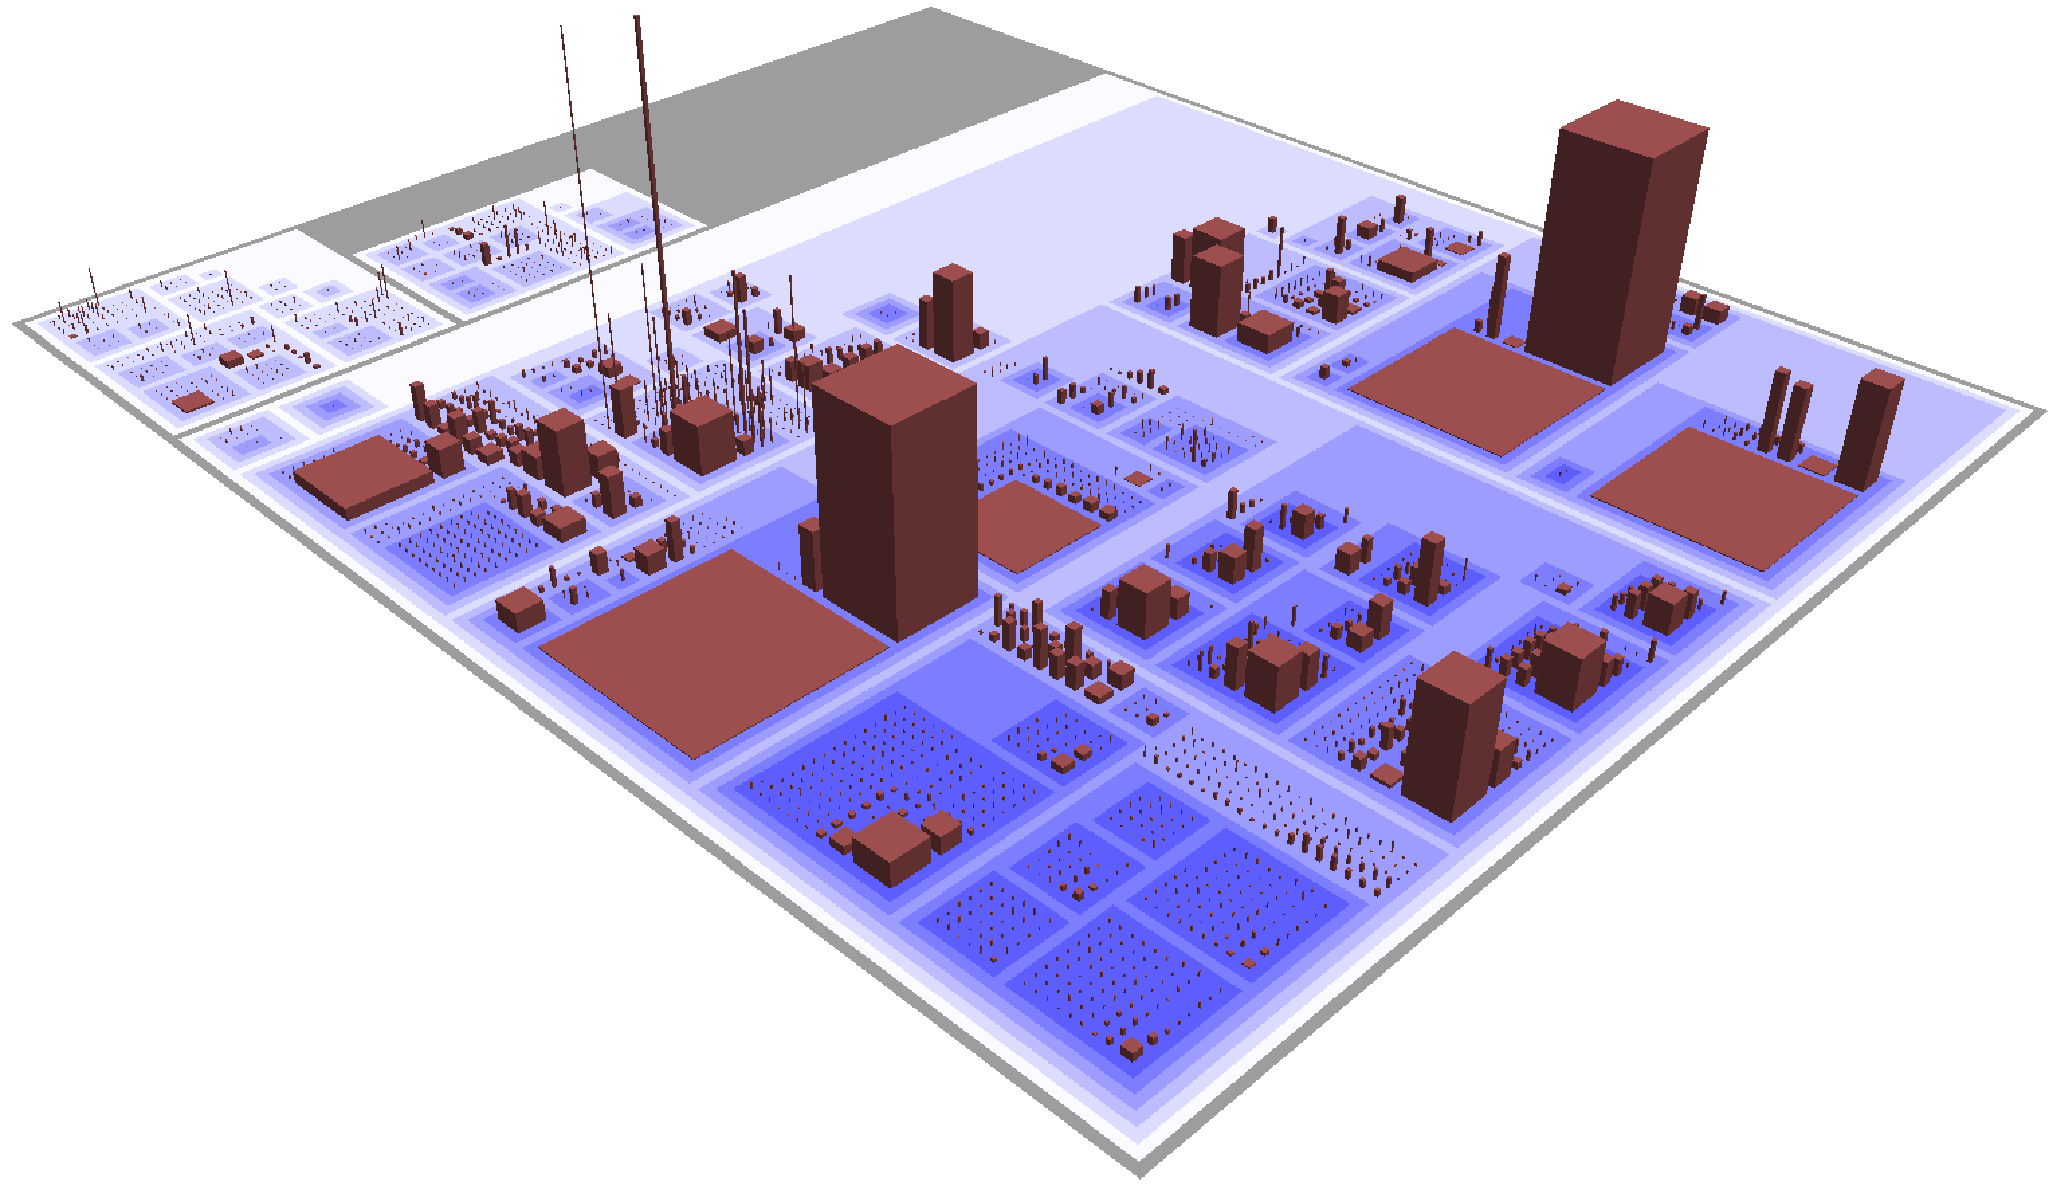
\includegraphics[width=\textwidth]{figures/code-city}
   \subcaption{CodeCity von ArgoUML \cite{wettel2008visual}} \label{fig:code-city}
  \end{subfigure}
  \hfill
  \begin{subfigure}[b]{\fwidth}
  	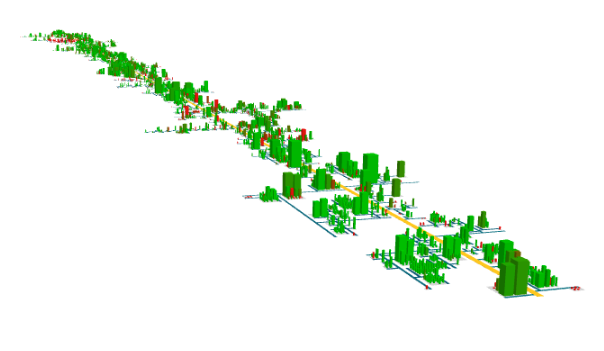
\includegraphics[width=\textwidth]{figures/softvis3d}
  	\subcaption{SoftVis3D mit Evostreet Layout} \label{fig:softvis3d}
  \end{subfigure}
  \hfill
  \vspace{1em}
  \begin{subfigure}[b]{\fwidth}
  	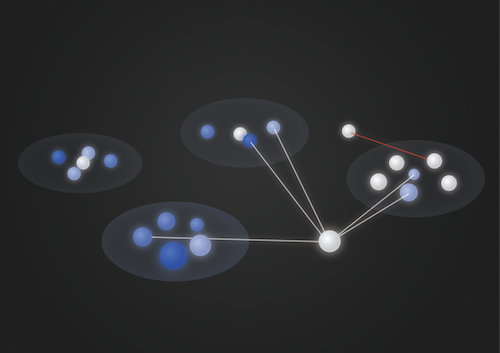
\includegraphics[width=\textwidth]{figures/code-universe}
  	\subcaption{Entwurf eines CodeUniverse} \label{fig:code-universe}
  \end{subfigure}
  \hfill
  \begin{subfigure}[b]{\fwidth}
  	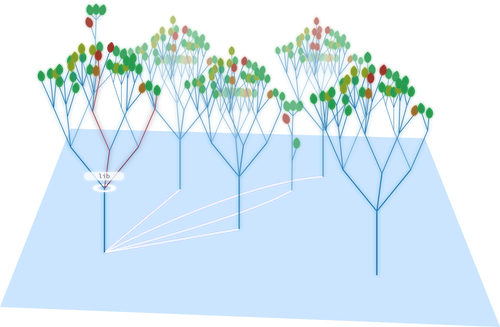
\includegraphics[width=\textwidth]{figures/code-leaves}
  	\subcaption{Erster Entwurf von CodeLeaves} \label{fig:code-leaves}
  \end{subfigure}
  \caption{CodeLeaves und alternative Modelle} \label{fig:alternatives}
\end{figure}

\subsubsection*{SoftVis3D}
SoftVis3D greift das Konzept der CodeCity auf und visualisiert als Plugin für SonarQube\footnote{SonarQube ist eine open-source Plattform für statische Code-Qualität, \url{https://www.sonarqube.org/}} Projekte direkt im Browser. Durch die direkte Anbindung an SonarQube, ist SoftVis3D hoch konfigurierbar und kann alle Metriken darstellen, die auch in SonarQube zur Verfügung. Neben dem \emph{District-Layout}, wie es in der CodeCity verwendet wird, unterstützt SoftVis3D darüber hinaus auch des \emph{Evostreet-Layout}, das ursprünglich in \cite{steinbruckner2013consistent} für die Evolution einer Software entworfen wurde. In diesem Layout, wie es in Abbildung \ref{fig:softvis3d} zu sehen ist, werden Pakete als Straßen dargestellt.

Die Evolution wird von SoftVis3D trotz Evostreet-Layout jedoch nicht unterstützt. Bei Die Abhängigkeiten wurde in früheren Versionen aggregiert dargestellt. Dafür wurden Pakete im Distrikt-Layout in übereinander liegenden Ebenen abgebildet und für $\Psi$ (vgl. Definition \ref{def:aggregation}) ein Hilfsgebäude benutzt, dass zu der darüberliegenden Ebene führt. Dadurch ging jedoch die Stadt-Metapher und die Übersichtlichkeit verloren. Die Dynamik kann in SoftVis3D ebenfalls nicht visualisiert werden. Die verwendete Technologie ist zwar mit \emph{WebGL} für den Browser State of the Art, aber für die HoloLens aktuell noch nicht sinnvoll einsetzbar \cite{puetz2017softwarevisualisierung}.

\subsubsection*{CodeUniverse}

Im Zuge der der Studie \cite{puetz2017softwarevisualisierung} wurde eine weitere Metapher evaluiert. Ähnlich wie in der Arbeit \cite{graham2004solar, balzer2004software}, wird die Software als Universum dargestellt. Die Softwareartefakte in Paketen gruppieren sich als Sterne in Galaxien. Statische Metriken können dann als Farbe und Größe der Sterne widergespiegelt werden. So können "`weiße Zwerge"' bis hin zu "`roten Riesen"' entstehen.

Das CodeUniverse ist für statische Metriken gut geeignet. Auch die Evolution ist mit der Entstehung von neuen Sternen und Galaxien gut vorstellbar. Die Struktur der Software ist zwar mit der Gruppierung der Sterne gegeben, aber weniger offensichtlich wie andere Konzepte. Bei der Visualisierung der Abhängigkeiten stößt das CodeUniverse aber an seine Grenzen. Durch direkte Verbindungen zwischen den Sternen lassen sich zwar Abhängigkeiten darstellen, aber bei großen Software-Systemen würde das schnell im Chaos enden. Auch in \cite{balzer2004software} wird beschrieben, dass eine übersichtliche Darstellung von Abhängigkeiten nur durch deren Aggregation erreicht werden kann. Deshalb wird in \cite{balzer2004software} ein Konzept entworfen, dass die Softwareartefakte mit einem \emph{"`hierarchischem Netz"'} verbindet. Dieses ist nichts anderes als die vorhandene Baumstruktur der Software und hat mit der Metapher des Universums auch nichts mehr zu tun. Folglich wären wir wieder bei dem neuen Konzept CodeLeaves angelangt.


\subsubsection*{Vorteile von CodeLeaves gegenüber anderen 3D Softwarevisualisierungen}
Die betrachteten Alternativen und weitere, haben gemein, dass sie zum einen Struktur, Dynamik und Evolution nicht vereinen. Zum anderen können Abhängigkeiten oder dynamische Aufrufe zwischen Softwareartefakten nicht ohne Verlust der Übersichtlichkeit angezeigt werden. CodeLeaves soll alle drei Kategorien der Softwarevisualisierung unterstützen und ist bei der Visualisierung der Struktur und der Abhängigkeiten den Alternativen überlegen. Durch die Baumstruktur, wie er auch in der Code-Base vorhanden ist, wird die Paket-Struktur eins zu eins wiedergegeben. Die aggregierten Abhängigkeiten lehnen sich an die Struktur an und beeinflussen diese nicht negativ. Durch das Wurzelgeflecht und die Spinnweben wird die Dreidimensionalität optimal ausgenutzt.

\section{Anforderungen an CodeLeaves}
\label{sec:requirements}

Die Umfrage, die in Abschnitt \ref{sec:comparison} vorgestellt wurde, ergab einen gutes Stimmungsbarometer über die Wünsche im Bezug auf zu visualisierend Informationen. In diesem Abschnitt soll genauer auf die Anforderungen an einen Software-Wald eingegangen werden. Dazu wurden von der QAware zwei Experten der Softwareanalyse zu diesem Thema befragt, um Userstories für CodeLeaves zu sammeln.

Aus der dynamischen Analyse wurde der promovierende Performance-Analyst F. Lautenschlager befragt. Dieser erarbeitete im Zuge seiner Dissertation eine hochperformante Zeitreihendatenbank zur Speicherung und Auswertung von dynamischen Daten einer Software und ist Experte auf diesem Gebiet.

Als Experte der statischen Analyse wurde J. Weigend befragt. Dieser ist Chefarchitekt, Geschäftsführer und Mitgründer der QAware. Er studierte Informatik mit Schwerpunkt "Verteilte Systeme" an der Hochschule Rosenheim und hält dort seit 2001 Vorlesungen \cite{qaware2017johannes}.

Im Folgenden werden die Gespräche mit den beiden Experten unter Anwendung der Methoden aus \cite{cohn2004user} in Userstories und dazugehörige Akzeptanzkriterien zusammengefasst. Zum Großteil überschneiden sich die Userstories mit der Umfrage aus Abschnitt \ref{sec:comparison}, was für eine gute Übereinstimmung der eingeholten Informationen spricht.

Zunächst betrachten wir die Userstories von Lautenschlager.
\begin{userstory}{Dynamische Metriken}
  Als \textit{Performance-Analyst}\\
  möchte ich \textit{Funktionsaufrufe, deren Antwortzeiten, Laufzeitfehler und Resourcen-Auslastung visualisiert haben},\\
  um \textit{das Laufzeitverhalten der Software explorativ bewerten zu können.}
\end{userstory}
  
\newcommand{\tableheader}{
\endfirsthead
\multicolumn{2}{l}{\small \tablename\ \thetable\ -- \textit{Fortsetzung von vorheriger Seite}} \\
\hline
  \endhead
  \hline
  \endlastfoot
  \hline
\multicolumn{2}{r}{\textit{\small Fortsetzung auf nächster Seite...}} \\
\endfoot
\hline
}
\renewcommand{\arraystretch}{1.5}
\begin{tabularx}{\textwidth}{lX}
	\caption{Akzeptanzkriterien zu Userstory 1}\label{tab:static-metrics} \\
	\tableheader
    1 & Antwortzeiten und Laufzeitfehler können als Metrik auf die Farbe der Blätter angewandt werden.\\
    2 & Wenn ich ein Blatt auswähle, dann kann ich die genaue Zahl der gerade betrachteten Metrik sehen.\\
    3 & Wenn ich ein Blatt auswähle, kann ich sehen wohin von dieser Klasse Aufrufe hin- bzw. eingehen.\\
    4 & Die Dicke einer Verbindung (d.h. ein Stück Ast oder Wurzel) zeigt mir die Anzahl der Aufrufe zwischen Anfang und Ende der Verbindung.\\
    5 & Wenn ich eine Verbindung anklicke, dann kann ich sehen, welche Klassen von dieser Verbindung betroffen sind.\\
    6 & Wenn ich eine Verbindung anklicke, dann kann ich sehen in welche Richtung die meisten betroffenen Verbindungen gehen.\\
    7 & Wenn ich den Wald betrachte, dann kann ich die Änderung der Ressourcen-Auslastung erkennen.
\end{tabularx}

\begin{userstory}{Zustand der Software}
  Als \textit{Systemverantwortlicher}\\
  möchte ich \textit{auf einen Blick den Zustand meiner Software erkennen},\\
  um \textit{bei Bedarf agieren zu können}.
\end{userstory}

\begin{tabularx}{\textwidth}{lX}
	\caption{Akzeptanzkriterien zu Userstory 2}\label{tab:static-metrics} \\
	\tableheader
    1 & Wenn ich die Laubfarbe des Waldes betrachte, dann möchte ich eine möglichst gute Gesamtübersicht über die ausgewählte Metrik haben.\\
    2 & Wenn ich die Laubfarbe des Waldes betrachte, dann kann ich Ausreißer der ausgewählten Metrik gut erkennen.\\
    3 & Die Struktur der Bäume ist möglichst übersichtlich und hat keine Überlappungen.
\end{tabularx}

\begin{userstory}{Kopplung und Struktur}
  Als \textit{Softwarearchiteckt}\\
  möchte ich \textit{die Kopplung und Struktur einer großen Software sehen},\\
  um \textit{die Zusammenhänge zu verstehen}.
\end{userstory}

\begin{tabularx}{\textwidth}{lX}
	\caption{Akzeptanzkriterien zu Userstory 3}\label{tab:static-metrics} \\
	\tableheader
    1 & Die Paketstruktur entspricht der Struktur der Bäume.\\
    2 & Wenn ich die Verbindungen zwischen einzelnen Bäumen oder Verzweigungen betrachte, dann erkenne ich durch die Dicke, wie stark die Pakete aneinander gekoppelt sind.\\
    3 & Wenn ich ein Blatt auswähle, dann kann ich die ein- bzw. ausgehenden Abhängigkeiten hervorheben.\\
    4 & Wenn ich ein Blatt auswähle, dann kann ich Abhängigkeiten direkt als Spinnweben darstellen.\\
    5 & Wenn ich eine Verbindung auswähle, dann kann ich die von den Abhängigkeiten betroffenen Klassen hervorheben.\\
    6 & Wenn ich eine Verbindung auswähle, dann kann ich sehen wie viele Abhängigkeiten in welche Richtung fließen.\\
    7 & Wenn ich auswähle, dass zyklische Abhängigkeiten hervorgehoben werden, können diese direkt als Spinnweben im gesamten Wald dargestellt werden.
\end{tabularx}

\begin{userstory}{Code-Qualität}
  Als \textit{Softwarearchitekt}\\
  möchte ich \textit{Code-Qualität auf die Struktur abbilden können},\\
  um \textit{Anomalien und Qualitätsdefizite zu erkennen}.
\end{userstory}

\begin{tabularx}{\textwidth}{lX}
	\caption{Akzeptanzkriterien zu Userstory 4}\label{tab:static-metrics} \\
	\tableheader
    1 & Statische Metriken der Code-Qualität, wie z.B. Code-Coverage, kann auf die Farbe der Blätter angewandt werden.\\
    2 & Wenn ich die Laubfarbe des Waldes betrachte, dann kann ich Ausreißer der ausgewählten Metrik gut erkennen.
\end{tabularx}

\begin{userstory}{Code-Qualität}
  Als \textit{Softwarearchitekt}\\
  möchte ich \textit{einen intuitiven Drilldown haben},\\
  um \textit{die Zusammenhänge auf verschiedener Pakte-Ebene zu verstehen}.
\end{userstory}

\begin{tabularx}{\textwidth}{lX}
	\caption{Akzeptanzkriterien zu Userstory 5}\label{tab:static-metrics} \\
	\tableheader
    1 & Wenn ich eine Verbindung auswähle, dann kann ich das repräsentierte Paket als neuen Waldboden festlegen. \\
    2 & Wenn ich die Laubfarbe des Waldes betrachte, dann kann ich Ausreißer der ausgewählten Metrik gut erkennen.
\end{tabularx}

\chapter{Datenmodell}
\label{ch:data-model}
\section{Schichtenmodell}
\label{ch:data-layers}

Das Datenmodell für CodeLeaves nimmt einen zentralen Baustein ein, auf den sich die Implementierung stützt. Bei dem Entwurfsmuster sind einige Prinzipien zu beachten. Wie Buschmann et al. in \cite{frank2007pattern} beschreibt, ist das Pattern \textit{Layers} ein Grundprinzip bei Software-Architekturen. Durch die \textit{Separation of concerns} werden einzelnen Schichten voneinander getrennt und können so zum Beispiel später ausgetauscht werden:

``Using semi-independent parts also enables the easier exchange of individual parts at a later date.`` \cite{frank2007pattern}

Gerade bei der Visualisierung von abstrakten Daten, wie es eine Software ist, ist eine Schichtentrennung besonders wichtig. CodeLeaves hat das Ziel eine beliebige objektorientierte Software darstellen zu können. Da aber nicht für jede Programmiersprache CodeLeaves angepasst werden soll, ist hier die erste Trennungsschicht sinnvoll. Die Software sollte in ein Sprach-agnostisches Format gebracht werden, mit dem CodeLeaves weiter arbeitet. Der Transfer von der realen Software in deren Repräsentation, kann dann für beliebige Sprachen ausgetauscht werden.

Wie in \todo{link auf Abgrenzung} bereits festgehalten, soll der Schritt des Transfers der realen Software in deren Repräsentation nicht Schwerpunkt dieser Arbeit sein.

Die Einteilung in Schichten geht aber noch weiter. Das Modell CodeLeaves könnte neben Software prinzipiell auch jegliche anderen, hierarchisch strukturierten Informationen darstellen. Für die interne Datenhaltung wird deshalb für die \textit{Application logic} das Datenmodell weiter abstrahiert und in ein Format gebracht, dass sich stark an der Baumstruktur der Informatik orientiert. So könnten später auch leicht andere Datenquellen angebunden werden.

Die letzte Schicht ist die der \textit{Presentation}. Das Datenmodell für hierarchische Informationen muss für die Darstellung der Bäume weiter verarbeitet werden. Zum Beispiel muss für die rekursive Generierung der Bäume bekannt sein, wie groß die maximale \textit{Tiefe} der einzelnen Äste ist. Nur so kann das Paket mit der tiefsten Schachtelung auch sinnvoll als \textit{Stamm} des Baumes dargestellt werden. Auch die Aggregation der Verbindungen zwischen einzelnen Blättern findet in diesem Schritt statt, sodass in den Zeichenalgorithmen, mit denen die Bäume in Unity generiert werden, keine fachliche Logik mehr benötigt wird.

Das bedeutet auch diese Schicht könnte wieder ausgetauscht werden und unterschiedliche Zeichenalgorithmen könnten unterstützt werden.

In Abbildung \ref{fig:data-layers} ist die Beziehung der Datenmodelle in den drei relevanten Schichten abgebildet.

\begin{figure}[htb]
  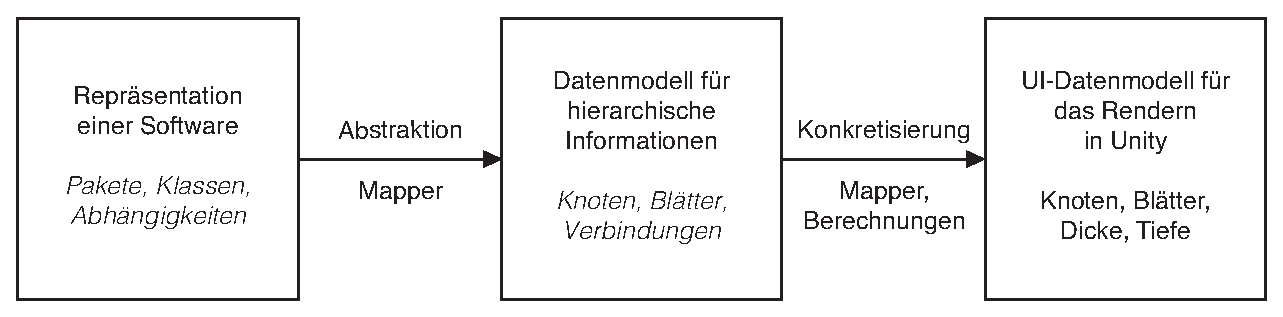
\includegraphics[width=\textwidth]{\figdir/data-layers}
  \caption{Schichten der Datenstrukturen}
  \label{fig:data-layers}
\end{figure}

\section{Datenmodell für die Repräsentation von Software}
\label{sec:software-model}

\section{Datenmodell für hierarchische Informationen}
\label{sec:hierarchical-model}

Das interne Datenmodell von CodeLeaves baut stark auf der Datenstruktur eines Baumes auf -- \textit{"`the most important nonlinear structures that arise in computer algorithms"'}\cite{knuth1973fundamental} -- das zum Beispiel in \cite{knuth1973fundamental, ernst2016grundkurs, gumm2009einfuehrung} definiert wird.

Da aber die Struktur von CodeLeaves zum Teil von der klassischen Definition abweicht und teilweise neue Bezeichnungen benötigt, betrachten wir daher einige Definitionen zur Baumstruktur, um diese an die Gegebenheiten von CodeLeaves anzupassen und führen neue Begriffe ein. Dabei sollen die Bezeichnungen für das interne Datenmodell, aber auch für die in Kapitel \ref{ch:modelling} behandelten Algorithmen Verwendung finden.

\subsection{Begriffsklärung}

\begin{itemize}
  \item Ein \textit{Baum} (engl.: \textit{tree}) besteht aus einer Menge von \textit{Knoten}, die so durch \textit{Kanten} verbunden sind, dass keine Kreise auftreten (Abgewandelt aus \cite{gumm2009einfuehrung, ernst2016grundkurs}).
  \item Ein \textit{Knoten} beinhaltet Informationen zu sich selbst und hat $0$ bis $n$ \textit{Kinder} (auch Nachfahren genannt, engl.: \textit{childs} oder \textit{descendant}).
  \item Ein Knoten mit keinen Kindern wird als \textit{Blatt} (engl.: \textit{leaf}) bezeichnet. Alle anderen Knoten heißen \textit{innere Knoten} (engl.: \textit{innerNode}) \cite{gumm2009einfuehrung}.
  \item Kinder des selben Knotens werden \textit{Geschwister} (engl.: \textit{siblings}) genannt.
\end{itemize}

Bei der klassischen Definition eines Baumes wird bei dem Knoten ohne Elternteil von der "`Wurzel"' gesprochen. Im Modell von CodeLeaves ist der unterste Knoten des Baumes jedoch noch durch eine Kante mit dem Waldboden verbunden. Darüber hinaus überschneidet sich die Bezeichnung von "`Wurzel"' mit den Verbindungen zwischen den einzelnen Bäumen, die bei der klassischen Definition nicht existieren. Deshalb wird für diesen speziellen Knoten eine neue Bezeichnung eingeführt.

\begin{itemize}
  \item Der unterste Knoten eines Baumes wird als \textit{Kronenansatz} (engl.: \textit{crown base}) bezeichnet.
  \item Alle Knoten bis auf den Kronenansatz haben genau einen Knoten als \textit{Elternteil} (auch Vorfahre genannt, engl.: \textit{parent} oder \textit{ancestor}).
\end{itemize}

Nachdem in den meisten Fällen Bäume in 2D nach unten wachsend dargestellt werden, was wahrscheinlich auf die Tatsache zurück zu führen ist, dass handschriftliche Diagramme tendenziell nach unten wachsend gezeichnet werden \cite{knuth1973fundamental}, wird bei Knoten auch oft von einer Tiefe gesprochen. Diese Bezeichnung wird beibehalten.

\begin{itemize}
  \item Die \textit{Tiefe} eines Knotens gibt an, wie viele Kanten er vom Kronenansatz aus entfernt liegt (Abgewandelt aus \cite{ernst2016grundkurs}).
  \item Die \textit{Höhe} (engl.: \textit{height}) eines Knoten beschreibt die maximale Tiefe aller Nachfahren.
\end{itemize}

Alle nachfolgenden Kanten und Knoten eines Knotens $A$ werden in der Literatur unterschiedlich bezeichnet. Es ist die Rede von "`Teilbaum"' \cite{ernst2016grundkurs} oder auch "`Unterbäumen"' \cite{gumm2009einfuehrung}. Wir definieren dafür einen dem 3D Modell besser entsprechenden Begriff.

\begin{itemize}
  \item Ein \textit{Ast} (engl.: \textit{branch}) sind alle nachfolgenden Kanten und Knoten des Knotens $A$ ausschließlich des Knotens $A$ selbst.
\end{itemize}

Bisher wurden Bezeichnungen aus einschlägiger Literatur verwendet oder abgeändert. Betrachten wir nun Elemente von CodeLeaves, die so nicht in der klassischen Definition einer Baumes vorkommen.

\begin{itemize}
  \item Der Kronenansatz ist durch die Kante namens \textit{Stamm} (engl.: \textit{trunk}) mit den \textit{Waldboden} (engl.: forest floor) verbunden.
  \item Der Schnittpunkt zwischen Stamm und Waldboden nennen wir \textit{Stammbasis} (engl.: \textit{trunk base}). Dieser ist jedoch kein Knoten und beinhaltet auch keine Informationen.
  \item Ein \textit{Wald} besteht aus einer disjunkten Menge an Bäumen und dem Waldboden.
  \item Ein Waldboden eines Waldes mit $n$ Bäumen besitzt $0$ bis $n!$ \textit{Wurzeln} (engl. \textit{roots}), die jeweils zwei Stammbasen miteinander verbinden.
\end{itemize}

\begin{figure}[htb]
  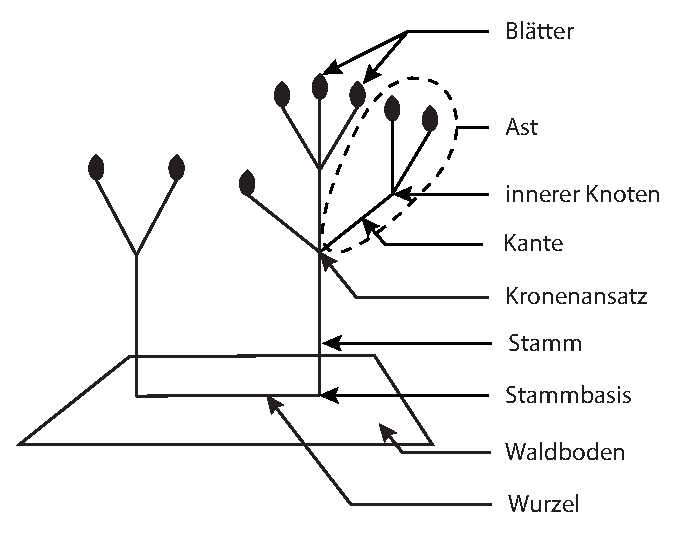
\includegraphics[width=.6\textwidth]{\figdir/naming}
  \caption{Bezeichnungen}
  \label{fig:naming}
\end{figure}


\begin{figure}[htb]
  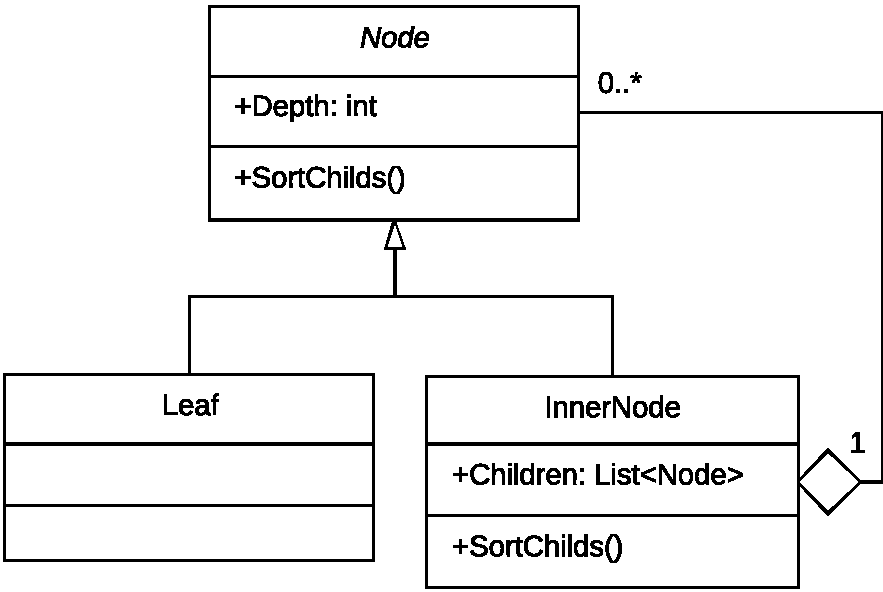
\includegraphics[width=.6\textwidth]{\figdir/ui-model}
  \caption{UI-Datenmodell}
  \label{fig:ui-model}
\end{figure}

% ----===== Chapter ====---- %
\chapter{Modellierung}
\label{ch:modelling}

\section{Generierung eines Baumes}

\subsection{Grundlegender Ansatz}
Für die Beschreibung der in diesem Kapitel betrachteten 

CodeLeaves steht und fällt mit der korrekten und übersichtlichen Darstellung der Baumstruktur. Durch Akzeptanzkriterium \todo{link auf Akzeptanz} ist die Struktur der Bäume so zu generieren, dass so viele Blätter wie möglich gleichzeitig im Blickfeld des Betrachters ist. Auf der anderen Seite gilt es wegen Akzeptanzkriterium \todo{link auf Akzeptanz} die Struktur übersichtlich und deswegen mit so wenig Überschneidungen wie möglich zu generieren.

Für die Generierung eines Baumes gibt es prinzipiell zwei verschiedene Ansätze. Ein Baum kann rekursiv von der Wurzel bis zu den Blättern generiert werden. Wir sprechen hier von der \textit{Bottom-up-Methode}. Wird bei den Blättern angefangen und rekursiv bis zur Wurzel miteinander verbunden, sprechen wir von der \textit{To-down-Methode}.

\subsubsection*{Bottom-up-Methode}
Bei dieser Methode wird ein Punkt im Raum vorgegeben und rekursiv für jeden folgenden Knoten

\subsubsection* {Top-down-Methode}


\subsection{Berechnung der Knoten Koordinaten}

Für das Anfügen einer neuen Kante oder einem Blatt an eine bestehende Kante müssen die Koordinaten des Knoten am Ende der bestehenden Kante berechnet werden.
 
Die Positionierung eines Knoten im Anschluss an den Stamm des Baumes ist trivial. Von der Position des Stammes auf dem Waldboden wird in y-Richtung die Länge des Stammes aufaddiert. Wächst der Baum z.B. auf dem Punkt $(0, 0, 0)$ und der Stamm hat eine länge von $h$, ergibt sich der Punkt für den Start aller direkt anschließenden Kanten mit $(0, h, 0)$. Für die Berechnung aller weiteren Punkte der Knoten müssen die Winkel der Äste jedoch miteinbezogen werden.
  
Wird eine Kante mit der Länge $l$ an einen Knoten angefügt, um die x-Achse mit dem Winkel $\theta$ geneigt und anschließend um die y-Achse mit den Winkel $\varphi$ rotiert, entsteht ein Kugelkoordinatensystem mit dem vorhandenen Knoten als Ursprung $O$, der y-Achse als Polachse, dem gesuchten Knoten als Punkt $P$, dem \emph{Polarwinkel} $\theta$ und dem \emph{Azimutwinkel} $\varphi$ \cite{papula2001mathematik}.

In Abbildung \ref{fig:node-calculation} ist die beschriebene Situation von der Seite und aus Vogelperspektive dargestellt.

\setlength{\fwidth}{.49\textwidth}
\begin{figure}[htb]
  \centering
  \begin{subfigure}[b]{\fwidth}
   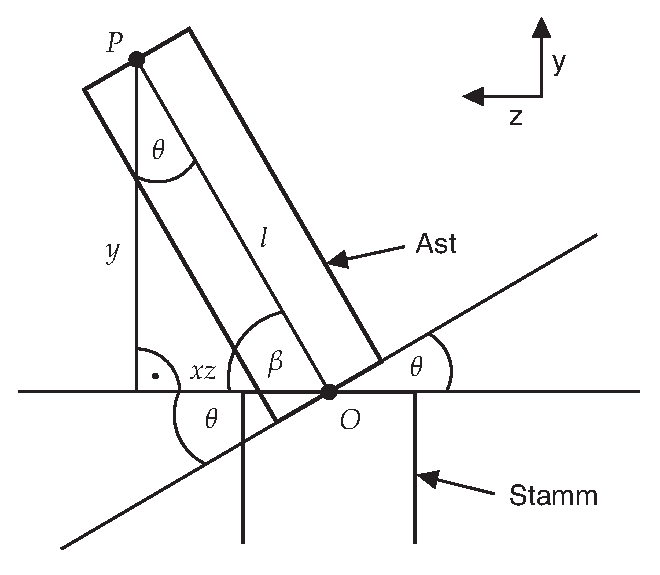
\includegraphics[width=\textwidth]{figures/yz-plane}
   \subcaption{Seitenansicht} \label{fig:yz-plane}
  \end{subfigure}
  \hfill
  \begin{subfigure}[b]{\fwidth}
  	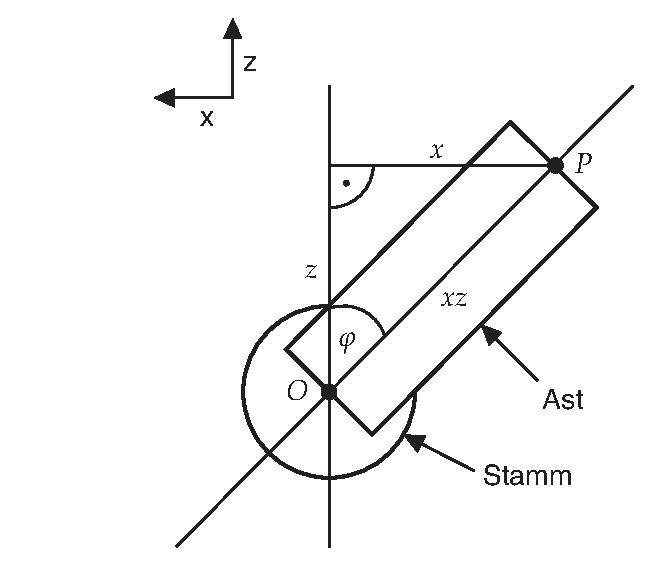
\includegraphics[width=\textwidth]{figures/xz-plane}
  	\subcaption{Vogelperspektive} \label{fig:xz-plane}
  \end{subfigure}
  \caption{Berechnung der Koordinaten eines neuen Knotens} \label{fig:node-calculation}
\end{figure}

Die Koordinaten $(l, \theta, \varphi)$ müssen in das kartesische Koordinatensystem umgerechnet werden. Dies wird durch folgende Formel erreicht:

\begin{equation}
  \vec{k} = 
  \begin{pmatrix}
    sin(\varphi) \cdot cos(\theta) \cdot l\\
    cos(\theta) \cdot l\\
    cos(\varphi) \cdot cos(\theta) \cdot l
  \end{pmatrix}
\end{equation}


In Unity spiegelt sich diese Formel in der Funktion \texttt{AddNode}, wie sie in Listing \ref{lst:addnode} zu sehen ist, wieder.

\begin{codesnippet}{Hinzufügen eines Knotens an eine Kante}{lst:addnode}
private static void AddNode(Transform branch, 
                            Transform edge, 
                            float edgeLength)
{
    var node = new GameObject("Node");
    node.transform.parent = branch;

    var theta = DegreeToRadian(edge.eulerAngles.x);
    var phi = DegreeToRadian(edge.eulerAngles.y);

    var y = (float) Math.Cos(theta) * edgeLength;
    var xz = (float) Math.Sin(theta) * edgeLength;
    var x = (float) Math.Sin(phi) * xz;
    var z = (float) Math.Cos(phi) * xz;

    node.transform.localPosition = new Vector3(x, y, z);
}
\end{codesnippet} 

%\tdplotsetmaincoords{60}{110}
%
\pgfmathsetmacro{\rvec}{1}
\pgfmathsetmacro{\thetavec}{30}
\pgfmathsetmacro{\phivec}{60}
%
\begin{tikzpicture}[scale=7,tdplot_main_coords]

\coordinate (O) at (0,0,0);
\draw[dashdotted,->] (0,0,0) -- (1,0,0) node[anchor=north east]{$z$};
\draw[dashdotted,->] (0,0,0) -- (0,1,0) node[anchor=north west]{$x$};
\draw[dashdotted,->] (0,0,0) -- (0,0,1) node[anchor=south]{$y$};

\tdplotsetcoord{P}{\rvec}{\thetavec}{\phivec}
\coordinate (E) at (Pz);

\draw[thick] (O) node[point,label=above left:$O$]{} -- node[left=3pt]{$h$} (E) node[point,label=above left:$E$]{};
\draw[thick] (O) -- node[below right]{$l$} (P) node[point,label=above right:$P$]{};
\draw (E) -- node[above right]{$a_n$} (P);
\draw[dashed] (O) -- (Pxy);
\draw[dashed] (P) -- (Pxy);
%\draw[dashed] (P) -- (Pyz);
%\draw[dashed] (E) -- (Pyz);

\tdplotsetthetaplanecoords{\phivec}
\tdplotdrawarc[tdplot_rotated_coords]{(E)}{0.1}{90}%
    {180}{above left}{$\cdot$}
\tdplotdrawarc{(O)}{0.2}{0}{\phivec}{anchor=north}{$\varphi$}
\tdplotdrawarc[tdplot_rotated_coords]{(0,0,0)}{0.3}{0}%
    {\thetavec}{anchor=south west}{$\theta$}
    
\end{tikzpicture}

%%Angle Definitions
%%-----------------
%
%%set the plot display orientation
%%synatax: \tdplotsetdisplay{\theta_d}{\phi_d}
%\tdplotsetmaincoords{0}{0}
%
%%define polar coordinates for some vector
%\pgfmathsetmacro{\rvec}{.8}
%\pgfmathsetmacro{\thetavec}{30}
%\pgfmathsetmacro{\phivec}{60}
%
%%start tikz picture, and use the tdplot_main_coords style to implement the display 
%%coordinate transformation provided by 3dplot
%\begin{tikzpicture}[scale=5, tdplot_main_coords]
%
%%set up some coordinates 
%%-----------------------
%\coordinate (O) at (0,0,0);
%
%%determine a coordinate (P) using (r,\theta,\phi) coordinates.  This command
%%also determines (Pxy), (Pxz), and (Pyz): the xy-, xz-, and yz-projections
%%of the point (P).
%%syntax: \tdplotsetcoord{Coordinate name without parentheses}{r}{\theta}{\phi}
%\tdplotsetcoord{P}{\rvec}{\thetavec}{\phivec}
%
%%draw figure contents
%%--------------------
%
%%draw the main coordinate system axes
%\draw[thick,->] (0,0,0) -- (1,0,0) node[anchor=north east]{$x$};
%\draw[thick,->] (0,0,0) -- (0,1,0) node[anchor=north west]{$y$};
%\draw[thick,->] (0,0,0) -- (0,0,1) node[anchor=south]{$z$};
%
%%draw a vector from origin to point (P) 
%\draw[-stealth,color=red] (O) -- (P);
%
%%draw projection on xy plane, and a connecting line
%\draw[dashed, color=red] (O) -- (Pxy);
%\draw[dashed, color=red] (P) -- (Pxy);
%
%%draw the angle \phi, and label it
%%syntax: \tdplotdrawarc[coordinate frame, draw options]{center point}{r}{angle}{label options}{label}
%\tdplotdrawarc{(O)}{0.2}{0}{\phivec}{anchor=north}{$\phi$}
%
%
%%set the rotated coordinate system so the x'-y' plane lies within the
%%"theta plane" of the main coordinate system
%%syntax: \tdplotsetthetaplanecoords{\phi}
%\tdplotsetthetaplanecoords{\phivec}
%
%%draw theta arc and label, using rotated coordinate system
%\tdplotdrawarc[tdplot_rotated_coords]{(0,0,0)}{0.5}{0}{\thetavec}{anchor=south west}{$\theta$}
%
%%draw some dashed arcs, demonstrating direct arc drawing
%\draw[dashed,tdplot_rotated_coords] (\rvec,0,0) arc (0:90:\rvec);
%\draw[dashed] (\rvec,0,0) arc (0:90:\rvec);

%set the rotated coordinate definition within display using a translation
%coordinate and Euler angles in the "z(\alpha)y(\beta)z(\gamma)" euler rotation convention
%syntax: \tdplotsetrotatedcoords{\alpha}{\beta}{\gamma}
%\tdplotsetrotatedcoords{\phivec}{\thetavec}{0}

%translate the rotated coordinate system
%syntax: \tdplotsetrotatedcoordsorigin{point}
%\tdplotsetrotatedcoordsorigin{(P)}

%use the tdplot_rotated_coords style to work in the rotated, translated coordinate frame
%\draw[thick,tdplot_rotated_coords,->] (0,0,0) -- (.5,0,0) node[anchor=north west]{$x'$};
%\draw[thick,tdplot_rotated_coords,->] (0,0,0) -- (0,.5,0) node[anchor=west]{$y'$};
%\draw[thick,tdplot_rotated_coords,->] (0,0,0) -- (0,0,.5) node[anchor=south]{$z'$};

%WARNING:  coordinates defined by the \coordinate command (eg. (O), (P), etc.)
%cannot be used in rotated coordinate frames.  Use only literal coordinates.  

%draw some vector, and its projection, in the rotated coordinate frame
%\draw[-stealth,color=blue,tdplot_rotated_coords] (0,0,0) -- (.2,.2,.2);
%\draw[dashed,color=blue,tdplot_rotated_coords] (0,0,0) -- (.2,.2,0);
%\draw[dashed,color=blue,tdplot_rotated_coords] (.2,.2,0) -- (.2,.2,.2);

%show its phi arc and label
%\tdplotdrawarc[tdplot_rotated_coords,color=blue]{(0,0,0)}{0.2}{0}{45}{anchor=north west,color=black}{$\phi'$}

%change the rotated coordinate frame so that it lies in its theta plane.
%Note that this overwrites the original rotated coordinate frame
%syntax: \tdplotsetrotatedthetaplanecoords{\phi'}
%\tdplotsetrotatedthetaplanecoords{45}

%draw theta arc and label
%\tdplotdrawarc[tdplot_rotated_coords,color=blue]{(0,0,0)}{0.2}{0}{55}{anchor=south west,color=black}{$\theta'$}

%\end{tikzpicture}

%\end{document}

\section{Positionierung der Bäume}

\section{Berechnung der aggregierten Verbindungen}

% ----==== Chapter ====---- %
\chapter{Interaktionskonzept}
\label{ch:interaction}
\chapter{Zusammenfassung und Ausblick}
\label{ch:conclusion}
		